\Variant{01.12.2024 (2-smena)}
\QQ{1}{$8\cdot40^{45}\cdot36^2\cdot625^{25}\cdot216$ neça xonali son?
\Opts{$149$}{$148$}{$147$}{$150$}}
\QQ{2}{$\dfrac1{30}+\dfrac1{60}+\dfrac1{100}+\dfrac1{150}+\dfrac1{210}$ ni hisoblang.
\Opts{$\dfrac1{15}$}{$\dfrac1{14}$}{$\dfrac2{19}$}{$\dfrac1{90}$}}
\QQ{3}{$A$ va $B$ şaharlardan ikkita turist $C$ şaharga yölga çiqdi. Agar $A$ va $B$ şahardagi turistlar bir-biriga qarab yursa $t_1$ vaqtda uçraşadi. Ikkita turist $C$ şaharga $t_2$ vaqtda birga yetib boradi. Turistlarning tezliklari köpaytmasini toping.
\qfig{\begin{tikzpicture}[scale=1,font=\small]
\draw (0,0)--(4.6,0); \fill (0,0) circle (1.5pt); \fill (2,0) circle (1.5pt); \fill (4.6,0) circle (1.5pt);
\draw[{Stealth[length=4pt]}-{Stealth[length=4pt]}] (0.1,0.3)--(1.9,0.3); \node[above] at (1,0.3) {$S$};
\node[below] at (0,0) {$A$}; \node[below] at (2,0) {$B$}; \node[below] at (4.6,0) {$C$};
\end{tikzpicture}}
\Opts{$\dfrac S2\left(\dfrac1{t_1}+\dfrac1{t_2}\right)$}{$\dfrac S2\left(\dfrac1{t_1}-\dfrac1{t_2}\right)$}{$\dfrac{S^2}4\left(\dfrac1{t_1^2}-\dfrac1{t_2^2}\right)$}{$S\left(\dfrac1{t_1^2}-\dfrac1{t_2^2}\right)$}}
\QQ{4}{Bir oilaning oylik maoşi $15\,000\,000$ söm. Uning $60\%$i oilaviy harajatlarga sarflanadi. Qolgan pulning $30\%$ini bankka omonatga qöyadi. Oila bankka neça söm pul qöyadi?
\Opts{$1\,800\,000$}{$2\,000\,000$}{$2\,500\,000$}{$2\,200\,000$}}
\QQ{5}{$a\cdot b=3^4\cdot5^2\cdot7^2\cdot11$ bölsa, EKUB$(a;\,b)$ ning eng katta qiymatini toping.
\Opts{$105$}{$315$}{$195$}{$1025$}}
\QQ{6}{Hisoblang:
\[\tg\frac\pi4+\sqrt3\sin\frac{7\pi}3\]
\Opts{$1$}{$1{,}5$}{$2$}{$2{,}5$}}
\QQ{7}{Kamayuvçi arifmetik progressiyada $a_1+a_3+a_5=15$ va $a_2^2+a_3^2+a_4^2=83$ bölsa, $a_{13}=\ ?$
\Opts{$25$}{$-17$}{$-15$}{$15$}}
\QQ{8}{Hisoblang:
\[\sqrt[3]{54+30\sqrt3}+\sqrt[3]{54-30\sqrt3}\]
\Opts{$3$}{$9$}{$6$}{$18$}}
\QQ{9}{$|x+2|+|x+5|=9+|x-4|$ tenglama neçta haqiqiy ildizga ega?
\Opts{$1$ ta}{$2$ ta}{$3$ ta}{Haqiqiy yeçimga ega emas}}
\QQ{10}{$6$ ta haddan iborat bölgan geometrik progressiyada dastlabki uçta hadi yiğindisi $26$ ga, oxirgi uçta hadi yiğindisi $702$ ga teng bölsa, maxrajini toping.
\Opts{$8$}{$6$}{$2$}{$3$}}
\QQ{11}{$a$ ning qanday qiymatida $\sqrt{25-x^2}=a$ tenglama haqiqiy ildizga ega?
\Opts{$[0;\,5]$}{$[0;\,25]$}{$(0;\,25)$}{$(0;\,5)$}}
\QQ{12}{$7^a=6$, $6^b=12$ bölsa, $\log_{81}98\sqrt3$ ni $a$ va $b$ orqali ifodalang.
\Opts{$\dfrac{4+ab}{16a-8ab}$}{$\dfrac{4+ab}{16a+8ab}$}{$\dfrac{4-ab}{16a+8ab}$}{$\dfrac{4-ab}{16a-8ab}$}}
\QQ{13}{$2\sin^2\left(x-\dfrac\pi3\right)-5\sin\left(x-\dfrac\pi3\right)+2=0$ tenglama $[-\pi;\,2\pi]$ oraliqda neçta yeçimga ega?
\Opts{$1$ ta}{$2$ ta}{$3$ ta}{$4$ ta}}
\QQ{14}{Tengsizlikni yeçing:
\[\frac{3^x-3^{x-2}}{3^x-2^x}>1+\left(\frac23\right)^x\]
\Opts{$(-\infty;\,0)$}{$\left(0;\,\log_{\frac23}\dfrac13\right)$}{$\left(-1;\,\log_{\frac23}\dfrac13\right)$}{$(-\infty;\,0)\cup\left(0;\,\log_{\frac23}\dfrac13\right)$}}
\QQ{15}{$\lg^2(x+1)=\lg(x-1)\cdot\lg(x+1)+2\lg^2(x-1)$ tenglamaning haqiqiy ildizlari köpaytmasini toping.
\Opts{$2$}{$3\sqrt2$}{$1$}{$\sqrt2$}}
\QQ{16}{Hisoblang:
\[\frac1{2\sqrt6+5}-5+2\sqrt6\]
\Opts{$4\sqrt6$}{$10$}{$0$}{$3\sqrt6$}}
\QQ{17}{Tengsizlikni yeçing:
\[-5\sqrt[4]x+\sqrt x+6\ge0\]
\Opts{$[0;\,16]$}{$[0;\,16]\cup[81;\,\infty)$}{$[16;\,81]$}{haqiqiy yeçimga ega emas}}
\QQ{18}{Soddalaştiring:
\[\left(\frac{8a^3+b^3}{4a^2-b^2}+b\right):\frac{a^2}{2a-b}\]
\Opts{$1$}{$2a-b$}{$4$}{$2a+b$}}
\QQ{19}{$\left(2x+1-\dfrac6x\right)\left(\dfrac{28}x-7+\left(\sqrt{-3-2x}\right)^2\right)\ge0$ tengsizlikning butun yeçimlari yiğindisini toping.
\Opts{$-22$}{$-25$}{$-27$}{$-28$}}
\QQ{20}{$y=x^2-\sqrt{9+x^2}$ funksiyaning eng kiçik butun qiymatini toping.
\Opts{$-4$}{$-2$}{$-1$}{$-3$}}
\QQ{21}{$h(x)=kx+l$ va $f(x)=mx+n$ ($k>0$) bölsa, $\dfrac{k+l}{m+n}=\ ?$
\qfig{\begin{tikzpicture}[x=0.6cm,y=0.42cm,font=\small]
\draw[-{Stealth[length=4pt]}] (-4.8,0)--(2.2,0) node[right] {$x$}; \draw[-{Stealth[length=4pt]}] (0,-1.8)--(0,7) node[left] {$y$};
\draw[thick,domain=-4.5:0.6,samples=60] plot (\x,{\x*\x+4*\x+3}); \draw (-4.8,2)--(2,2);
\node[below] at (-3,0) {$-3$}; \node[below left] at (-1,0) {$-1$}; \node[below right] at (0,2) {$2$}; \node[right] at (0,3.1) {$3$};
\node[right] at (0.6,2.6) {$y_2=h(x)-f(x)$}; \node[left] at (-0.4,6.3) {$y_1=h(x)\cdot f(x)$};
\end{tikzpicture}}
\Opts{$1$}{$2$}{$3$}{$4$}}
\QQ{22}{$f(x)=3^x\log_3(3x)$ bölsa, $f'(1)$ ni toping.
\Opts{$\dfrac{\ln^23+1}{\ln3}$}{$\dfrac{3\ln^23+3}{\ln3}$}{$\dfrac{3\ln^23-3}{\ln3}$}{$\dfrac{3\ln^23+1}{\ln3}$}}
\QQ{23}{$f(x)=\left|x^2+3x+2\right|$ va $g(x)=x+2$ funksiyalar bilan çegaralangan sohaning yuzini toping.
\Opts{$\dfrac12$}{$1$}{$\dfrac18$}{$2$}}
\QQ{24}{Rasmda $O$ markazli aylana bilan $ABCD$ kvadrat tasvirlangan. $O$ nuqta $AD$ tomonda yotadi. Agar $K$ va $L$ nuqtalar aylana va kvadratning kesişiş nuqtalari bölib, $OD=4$, $DL=2$ va $BC=6$ bölsa, $KL$ kiçik yoyning uzunligini toping.
\qfig{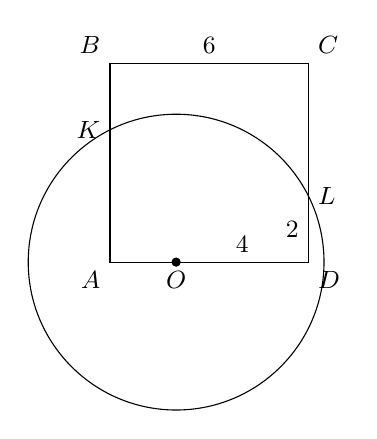
\begin{tikzpicture}[scale=0.42,font=\small]
\coordinate (O) at (0,0); \coordinate (A) at (-2,0); \coordinate (D) at (4,0); \coordinate (B) at (-2,6); \coordinate (C) at (4,6); \coordinate (K) at (-2,4); \coordinate (L) at (4,2);
\draw (A)--(B)--(C)--(D)--cycle; \draw (O) circle (4.472); \fill (O) circle (4pt);
\node[below left] at (A) {$A$}; \node[above left] at (B) {$B$}; \node[above right] at (C) {$C$}; \node[below right] at (D) {$D$}; \node[below] at (O) {$O$}; \node[left] at (K) {$K$}; \node[right] at (L) {$L$};
\node[above] at (1,6) {$6$}; \node[above] at (2,0) {$4$}; \node[left] at (4,1) {$2$};
\end{tikzpicture}}
\Opts{$\sqrt3\,\pi$}{$2\pi$}{$\sqrt5\,\pi$}{$\sqrt6\,\pi$}}
\QQ{25}{$ABC$ uçburçakda $AB=5$, $BC=4$ va $AC=3$ ga teng. $C$ burçak uçidan $AB$ tomonga balandlik va bissektrisa tuşirilgan bölsa, ular orasidagi masofani toping.
\qfig{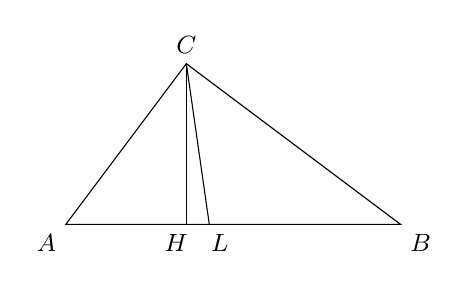
\begin{tikzpicture}[scale=0.85,font=\small]
\coordinate (A) at (0,0); \coordinate (B) at (5,0); \coordinate (C) at (1.8,2.4); \coordinate (H) at (1.8,0); \coordinate (L) at (2.143,0);
\draw (A)--(B)--(C)--cycle; \draw (C)--(H); \draw (C)--(L);
\node[below left] at (A) {$A$}; \node[below right] at (B) {$B$}; \node[above] at (C) {$C$}; \node[below] at (1.65,0) {$H$}; \node[below] at (2.3,0) {$L$};
\end{tikzpicture}}
\Opts{$\dfrac{13}{35}$}{$\dfrac{11}{35}$}{$\dfrac{17}{35}$}{$\dfrac{12}{35}$}}
\QQ{26}{$ABC$ töğri burçakli uçburçakka aylana şunday çizilganki, aylana $AB$ katetga urinib, şu katet qarşisidagi burçakdan ötadi. Aylana markazi $O$ nuqta $BC$ gipotenuzada joylaşgan, aylana gipotenuzani $E$ nuqtada kesib ötadi. Agar $BE=1$, $OC=4$ va $\angle BCD=\angle ACD$ bölsa, $O$ nuqtadan $DC$ tomongaça bölgan masofani toping.
\qfig{\begin{tikzpicture}[scale=0.55,font=\small]
\coordinate (B) at (0,0); \coordinate (E) at (1,0); \coordinate (O) at (5,0); \coordinate (C) at (9,0); \coordinate (D) at (1.8,2.4); \coordinate (A) at (3.24,4.32);
\draw (O) circle (4); \draw (A)--(B)--(C)--cycle; \draw (D)--(C); \fill (O) circle (3pt);
\draw ($(A)!0.45cm!(B)$)--($(A)!0.45cm!(B)!0.45cm!90:(B)$)--($(A)!0.45cm!(C)$);
\node[above] at (A) {$A$}; \node[left] at (B) {$B$}; \node[right] at (C) {$C$}; \node[above left] at (D) {$D$}; \node[below right] at (E) {$E$}; \node[below] at (O) {$O$};
\node[below] at (0.5,0) {$1$}; \node[below] at (3,0) {$4$}; \node[below] at (7,0) {$4$};
\end{tikzpicture}}
\Opts{$\dfrac{2\sqrt{10}}5$}{$\dfrac{3\sqrt{10}}5$}{$\dfrac{4\sqrt{10}}5$}{$\dfrac{\sqrt{10}}5$}}
\QQ{27}{$ABCD$ töğri burçakli trapetsiyaning kiçik asosi katta yon tomoniga teng, balandligi $4$ ga teng va katta diagonali $4\sqrt5$ ga teng bölsa, trapetsiya yuzini toping.
\qfig{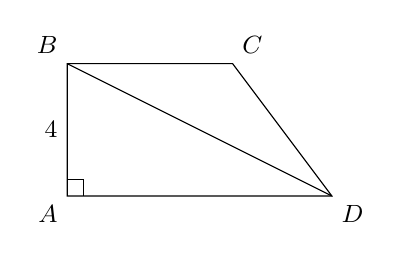
\begin{tikzpicture}[scale=0.42,font=\small]
\coordinate (A) at (0,0); \coordinate (B) at (0,4); \coordinate (C) at (5,4); \coordinate (D) at (8,0);
\draw (A)--(B)--(C)--(D)--cycle; \draw (B)--(D); \draw (0,0.5)--(0.5,0.5)--(0.5,0);
\node[below left] at (A) {$A$}; \node[above left] at (B) {$B$}; \node[above right] at (C) {$C$}; \node[below right] at (D) {$D$}; \node[left] at (0,2) {$4$};
\end{tikzpicture}}
\Opts{$32$}{$35$}{$26$}{$24$}}
\QQ{28}{Tekislikda yotmagan $A$ nuqta orqali tekislikka $AH$ balandlik va $AM$ oğma tuşirilgan. Agar oğma va tekislik orasidagi burçak $37^\circ$ va $AH=6$ bölsa, $H$ uçidan $AM$ oğmagaça bölgan eng qisqa masofani toping. ($\cos37^\circ=0{,}8$ deb oling)
\Opts{$1{,}8$}{$3{,}6$}{$4{,}8$}{$2{,}4$}}
\QQ{29}{$ABC$ uçburçak yuzi $60$ ga teng. $\overrightarrow{BE}=-\dfrac12\overrightarrow{BA}$ bölsa, $ACE$ uçburçak yuzini toping.
\Opts{$30$}{$60$}{$90$}{$120$}}
\QQ{30}{Tomonlari soni $n$ juft son bölgan muntazam köpburçakning bir uçidan çiqqan eng katta va eng kiçik diagonallari orasidagi burçak $45^\circ$ ga teng. Muntazam köpburçak içki burçaklar yiğindisini toping.
\Opts{$1080^\circ$}{$1440^\circ$}{$720^\circ$}{$1800^\circ$}}
\QQ{31}{Böş töplamlar sonini toping. $R$ — haqiqiy sonlar töplami, $I$ — irratsional sonlar töplami.
\[1)\ \left\{x\mid x^2-\sqrt{10}+\pi=0;\ x\in R\right\}\qquad 2)\ \left\{x\mid x^2+1=0;\ x\in R\right\}\]
\[3)\ \left\{x\mid |x|=-3;\ x\in R\right\}\qquad 4)\ \left\{x\mid x^2+3x+2=0;\ x\in I\right\}\]
\Opts{$1$ ta}{$2$ ta}{$3$ ta}{$4$ ta}}
\QQ{32}{Tört xonali sonlar içidan raqamlari toq sonlardan iborat bölgan va $5$ ga karrali son böliş ehtimolligini toping.
\Opts{$\dfrac1{72}$}{$\dfrac1{36}$}{$\dfrac1{108}$}{$\dfrac15$}}
\QQ{33}{\Moslash{$O(0;0;0)$, $A(0;0;3)$ va $B\left(\sqrt2;\sqrt2;0\right)$ bölib, $D$ va $C$ nuqtalar mos ravişda $OX$ va $OY$ öqlarida joylaşgan. $OB$ kesma $OCD$ uçburçakning balandligi va medianasi böladi. ($\pi\approx3$ deb hisoblang)
\par\centering\begin{tikzpicture}[scale=0.8,font=\small]
\coordinate (O) at (0,0); \coordinate (A) at (0,2.1); \coordinate (D) at (1.6,-1.6); \coordinate (C) at (2.6,0.7); \coordinate (B) at (2.1,-0.45);
\draw[-{Stealth[length=4pt]}] (O)--(0,3) node[left] {$z$}; \draw[-{Stealth[length=4pt]}] (O)--(2.1,-2.1) node[right] {$x$}; \draw[-{Stealth[length=4pt]}] (O)--(3.6,0.97) node[right] {$y$};
\draw (D)--(C); \draw (O)--(B); \draw[dashed] (A)--(D); \draw[dashed] (A)--(C); \draw[dashed] (A)--(B);
\fill (A) circle (1.5pt); \fill (B) circle (1.5pt);
\node[left] at (A) {$A$}; \node[right] at (A) {$3$}; \node[left] at (O) {$O$}; \node[below left] at (D) {$D$}; \node[above] at (C) {$C$}; \node[right] at (B) {$B$};
\end{tikzpicture}}{A) $3$\par B) $4$\par C) $6$\par D) $12$\par E) $16$\par F) $24$}{$AOCD$ piramida hajmini toping.}{$AOB$ uçburçakning $AO$ tomoni atrofida $360^\circ$ ga aylantirişdan hosil bölgan jism hajmini toping.}{$OCD$ uçburçakning $CD$ tomoni atrofida $360^\circ$ ga aylantirişdan hosil bölgan jism hajmini toping.}}
\QQ{36}{$a$, $b$, $c$ sonlar $x^3-9x^2+11x-1=0$ tenglamaning haqiqiy ildizlari. $t=\sqrt a+\sqrt b+\sqrt c$ bölsa,
\AB{$a+b+c+abc+ab+bc+ac$ ni toping.}{$t^4-18t^2-8t$ ni hisoblang.}}
\QQ{37}{Quyidagi tenglama berilgan:
\[\sqrt{7+8\cos^2\frac{\pi x}{18}}=4\sin^2\frac{\pi x}{18}\]
\AB{$[0;\,18]$ oraliqdagi yeçimlar yiğindisini toping.}{$[20;\,30]$ oraliqdagi ildizlari sonini toping.}}
\QQ{38}{Agar $f(x)=\dfrac{x+3}{x-1}$ berilgan bölsa ($f^{-1}(x)$ — $f(x)$ funksiyaga teskari funksiya),
\AB{$f^{-1}(2)$ ni hisoblang.}{$f(x)=f^{-1}(x)$ tenglamaning ildizi böla olmaydigan neçta butun son bor?}}
\QQ{39}{Töğri burçakli trapetsiyaning içki sohasiga eng katta yuzli töğri törtburçak çizilgan. Töğri törtburçakning bir tomoni trapetsiyaning katta asosida yotadi. Trapetsiyaning asoslari $6$ va $16$ ga, balandligi $15$ ga teng.
\qfig{\begin{tikzpicture}[scale=0.22,font=\small]
\draw (0,0)--(16,0)--(6,15)--(0,15)--cycle; \fill[qfill] (0,0) rectangle (8,12); \draw (0,0) rectangle (8,12);
\draw (0,0)--(16,0)--(6,15)--(0,15)--cycle;
\node[below] at (8,0) {$16$}; \node[above] at (3,15) {$6$}; \node[left] at (0,7.5) {$15$};
\end{tikzpicture}}
\AB{Töğri törtburçak yuzini toping.}{Trapetsiya yuzidan töğri törtburçak yuzini ayirgandagi farqning modulini toping.}}
\QQ{40}{$f(x)$ funksiya uçun $f''(x)=12x^2+6x$, $f'(1)=9$ va $f(1)=5$ tengliklar örinli bölsa,
\AB{$f(0)$ ni hisoblang.}{$g(x)$ funksiya uçun $g(2024)=2$ va $g(2023)=3$ bölsa, $\displaystyle\int_{2023}^{2024}\left(g(x)+x\,g'(x)\right)dx$ ni hisoblang.}}
\QQ{41}{Rasmda $ABCD$ kvadrat va markazi $B$ nuqtada va radiusi $r$ ga teng aylana berilgan. $E$ nuqta $DB$ nurida, aylanada yotadi.
\qfig{\begin{tikzpicture}[scale=0.85,font=\small]
\coordinate (B) at (0,0); \coordinate (C) at (2,0); \coordinate (A) at (0,-2); \coordinate (D) at (2,-2); \coordinate (E) at (-1.414,1.414);
\fill[qfill] (E)--(C) arc (0:-90:2) --cycle;
\draw (B) circle (2); \draw (A)--(B)--(C)--(D)--cycle; \draw (E)--(C); \draw (E)--(A); \draw (E)--(D);
\node[above left] at (E) {$E$}; \node[above left] at (B) {$B$}; \node[right] at (C) {$C$}; \node[below] at (A) {$A$}; \node[right] at (D) {$D$};
\end{tikzpicture}}
\AB{Kvadrat içidagi böyalgan sohaning böyalmagan soha yuziga nisbatini toping.}{Agar $r=2$ bölsa, böyalgan soha yuzini toping.}}
\QQ{42}{$ABC$ töğri burçakli uçburçakning $AC$ va $BC$ katetlarida mos ravişda $D$ va $E$ nuqtalar şunday tanlab olinganki $AD=BC$ va $CD=BE$ tengliklar örinli bölsa,
\qfig{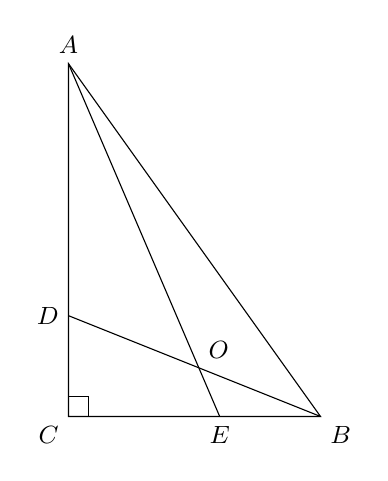
\begin{tikzpicture}[scale=0.32,font=\small]
\coordinate (C) at (0,0); \coordinate (A) at (0,14); \coordinate (B) at (10,0); \coordinate (D) at (0,4); \coordinate (E) at (6,0); \coordinate (O) at (5.172,1.931);
\draw (A)--(B)--(C)--cycle; \draw (A)--(E); \draw (D)--(B); \draw (0,0.8)--(0.8,0.8)--(0.8,0);
\node[above] at (A) {$A$}; \node[below right] at (B) {$B$}; \node[below left] at (C) {$C$}; \node[left] at (D) {$D$}; \node[below] at (E) {$E$}; \node[above right] at (O) {$O$};
\end{tikzpicture}}
\AB{$\angle AOD$ burçakni toping.}{$BC=10$ va $AE=2\sqrt{58}$ bölsa, $S_{ABC}$ ni hisoblang.}}
\QQ{43}{$ABCD$ parallelogrammning diagonallarida olingan $A_1$, $B_1$, $C_1$, $D_1$ va $E$ nuqtalar uçun $A_1E\parallel AD$ va $C_1E\parallel CD$ bölib, $AC:A_1C_1=5:3$ va $BD:B_1D_1=3:2$ nisbatlar örinli bölsa,
\qfig{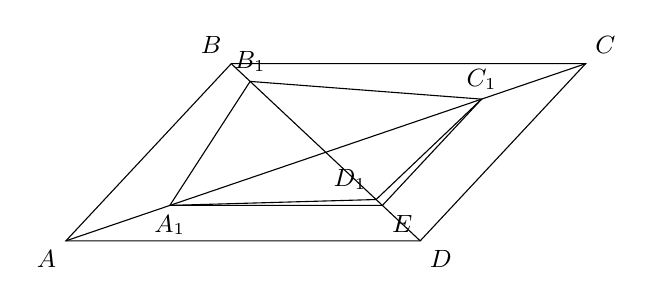
\begin{tikzpicture}[scale=0.75,font=\small]
\coordinate (A) at (0,0); \coordinate (D) at (6,0); \coordinate (B) at (2.8,3); \coordinate (C) at (8.8,3);
\coordinate (A1) at (1.76,0.6); \coordinate (C1) at (7.04,2.4); \coordinate (E) at (5.36,0.6); \coordinate (B1) at (3.12,2.7); \coordinate (D1) at (5.253,0.7);
\draw (A)--(B)--(C)--(D)--cycle; \draw (A)--(C); \draw (B)--(D);
\draw (A1)--(B1)--(C1)--(D1)--cycle; \draw (A1)--(E)--(C1);
\node[below left] at (A) {$A$}; \node[above left] at (B) {$B$}; \node[above right] at (C) {$C$}; \node[below right] at (D) {$D$};
\node[below] at (A1) {$A_1$}; \node[above] at (B1) {$B_1$}; \node[above] at (C1) {$C_1$}; \node[above left] at (D1) {$D_1$}; \node[below right] at (E) {$E$};
\end{tikzpicture}}
\AB{$\dfrac{S_{A_1C_1E}}{S_{ACD}}$ ni toping.}{$\dfrac{S_{A_1B_1C_1D_1}}{S_{ABCD}}$ ni toping.}}
\QQ{44}{Şarga, şar hajmining $\dfrac14$ qismini taşkil qiluvçi konus içki çizilgan. ($\pi\approx3$ deb oling)
\qfig{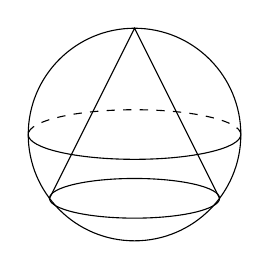
\begin{tikzpicture}[scale=0.9,font=\small]
\draw (0,0) circle (1.5); \draw (-1.5,0) arc (180:360:1.5 and 0.35); \draw[dashed] (1.5,0) arc (0:180:1.5 and 0.35);
\draw (-1.2,-0.9)--(0,1.5)--(1.2,-0.9); \draw (0,-0.9) ellipse (1.2 and 0.28);
\end{tikzpicture}}
\AB{$H_{\text{konus}}=\sqrt[3]{2+\sqrt5}$ va $H_{\text{konus}}>R_{\text{şar}}$ bölsa, şar hajmini toping.}{$R_{\text{şar}}=H_{\text{konus}}=\sqrt{3+2\sqrt2}$ bölsa, konusga içki çizilgan sfera sirtining yuzini toping.}}
\QQ{45}{Sirk karkasining eng baland nuqtasidan yergaça bölgan masofa $8$ ga, kengligi $20$ ga teng bölgan parabola şaklida. Karkas qulab ketmasligi uçun balandligi $6$ ga teng nuqtasida yerga tros tortilgan (tros parabolaga urinadi).
\qfig{\begin{tikzpicture}[scale=0.38,font=\small]
\draw (-4,0)--(21,0); \draw[thick,domain=0:20,samples=60] plot (\x,{8-0.08*(\x-10)^2});
\draw (-2.5,0)--(5,6); \draw[dashed] (5,0)--(5,6); \draw[dashed] (10,0)--(10,8);
\draw (-2.5,0)+(0:1.2) arc (0:38.66:1.2); \node at (-0.7,0.45) {\scriptsize$\alpha$};
\node[below] at (-2.5,0) {$D$}; \node[below] at (0,0) {$O$}; \node[below] at (5,0) {$B$}; \node[below] at (10,0) {$E$}; \node[below] at (20,0) {$K$};
\node[above left] at (5,6) {$A$}; \node[above] at (10,8) {$C$}; \node[right] at (5,3) {$6$}; \node[right] at (10,4) {$8$};
\draw[{Stealth[length=4pt]}-{Stealth[length=4pt]}] (0,-1.6)--(20,-1.6); \node[fill=white,inner sep=1pt] at (10,-1.6) {$20$};
\end{tikzpicture}}
\AB{$\tg\alpha$ ni toping.}{$OD$ ni toping.}}
\Javoblar{A B C A B D C C B D A A C B B C B C C D B B B C D A C C C A C A B D E}{%
\OK{36}{$21$}{$-37$}\OK{37}{$18$}{$2$ ta}\OK{38}{$5$}{$1$ ta}\OK{39}{$96$}{$69$}\OK{40}{$1$}{$-2021$}%
\OK{41}{$\dfrac\pi{4-\pi}$}{$2\sqrt2+\pi$}\OK{42}{$45^\circ$}{$70$}\OK{43}{$\dfrac9{25}$}{$\dfrac25$}\OK{44}{$4$}{$12$}\OK{45}{$0{,}8$}{$2{,}5$}}
